\chapter{Radare2 Framework}
\label{chapter:radare}

The Radare\cite{pancake2008rbook}\cite{pancake2009radare}\footnote{\url{https://github.com/radare/radare}} project started in 2006 as a forensics tool, built around a command line hexadecimal editor. Its goal was to provide a free and open source tool to search and recover data from hard-disks. With the open source community support, the project evolved and has grown into a complete framework for reverse engineering, exploiting, fuzzing, binary and data analysis.

In 2009 the framework was completely rewritten due to initial design limitations, thus the current Radare2\cite{maijin2016r2book}\footnote{\url{https://github.com/radare/radare2}} framework was born and continues to grow ever since with the support of the open source community.

\section{Framework Presentation}
\label{sec:presentation}

At its core the Radare2 framework is still a hexadecimal editor. However the full framework now contains also an assembler / disassembler, code / data analysis tools, graphing tools, scripting features and internal database among others.

One of the main advantages\footnote{Radare2 Comparison Table \url{http://rada.re/r/cmp.html}} Radare2 has over other reverse engineering tools or frameworks is its versatility, currently supporting over 30 different architectures and instruction sets\footnote{\url{https://en.wikipedia.org/wiki/Radare2\#Supported_architectures.2Fformats}} as well as over 15 different file formats.


All of these have led to the adoption of Radare2 in academia as well as software security researchers for forensics and analysis purposes, Capture The Flag teams across the globe and security-oriented personnel in general. Some of the main use cases include:
\begin{itemize}
	\item Static Analysis
	\item Dynamic Analysis
	\item Software exploitation
\end{itemize}

The framework also encourages a hands-on approach:
\begin{quote}"There is no formal documentation of r2 yet. Not all commands are compatible with radare1, so the best way to learn how to do stuff in r2 is by reading the examples from the web and appending '?' to every command you are interested in."
\end{quote}



\section{Architectural Overview}
\label{sec:architecture}

The Radare2 framework consists of multiple command-line utilities:
\begin{itemize}
	\item rabin2: tool for extracting information from executable binaries
	\item rasm2: the assembler / disassembler with multi-architecture support
	\item rahash2: hashing tool, supports different algorithms: MD4, MD5, CRC16, CRC32, SHA1, SHA256, SHA384, SHA512, etc.
	\item radiff2: binary diffing tool
	\item rafind2: pattern-search utility
	\item ragg2: compiler for high-level language
	\item rarun2: launcher for running different environments
	\item rax2: mathematic expression evaluator
	\item radare2: the core hexadecimal editor and debugger, integrates all of the above
\end{itemize}

\fig[scale=0.19]{src/img/r2arch.png}{img:r2arch}{Radare2 Module Architecture}

\section{Key Features}
\label{sec:features}

There are several specific key features and tools which Radare2 provides that make it the ideal starting point for this project.

\subsection{Gadget Finder}

The framework already includes a tool for ROP gadget searching (\labelindexref{Figure}{fig:gadgetsearch}). This comes with integrated support for Regular Expression matching as well as JSON formatting options for portability.

\begin{figure}[htp]%[!tbp]
	\centering
	\subfloat[Basic search]{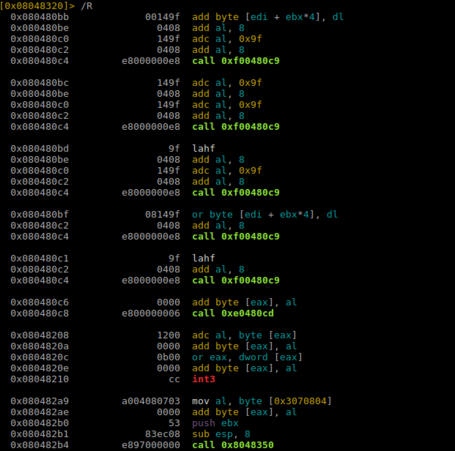
\includegraphics[width=0.45\textwidth]{src/img/gadgets4.png}\label{fig:f1}}
	\hfill
	\subfloat[Regex search]{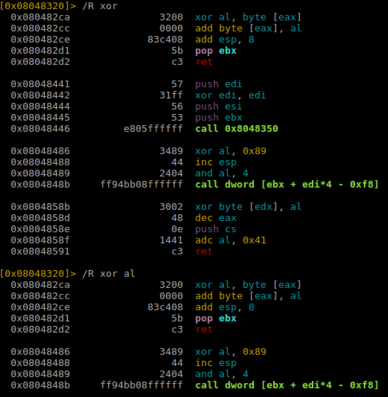
\includegraphics[width=0.45\textwidth]{src/img/gadgetsRegex.png}\label{fig:f2}}
	% \hfill
	\caption{ROP Gadget Search}
	\label{fig:gadgetsearch}
\end{figure}

\subsection{ESIL}

ESIL stands for ``Evaluable String Intermediate Language'' and can be used as an Intermediate Representation for Radare2. It provides a simple representation for every supported instruction set opcode and represents it as a combination of common operations performed by CPUs: binary arithmetic operations, memory loads and stores, syscalls etc. The complete ESIL instruction set aims for simplicity and robustness, a full description can be found in the Radare2 Book\cite{maijin2016r2book}.

By setting only one environment variable we can for example change the output of the disassembler from assembly to ESIL as seen in \labelindexref{Figure}{fig:disasEsil}.
% \todo{insert figure of pd call with esil}

\begin{figure}[htp]%[!tbp]
	\centering
	\subfloat[Disassemble without ESIL]{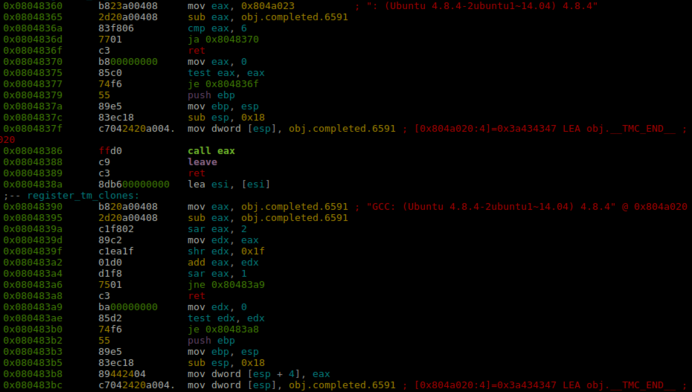
\includegraphics[width=0.49\textwidth]{src/img/disassemble.png}\label{fig:f1}}
	\hfill
	\subfloat[Disassemble with ESIL]{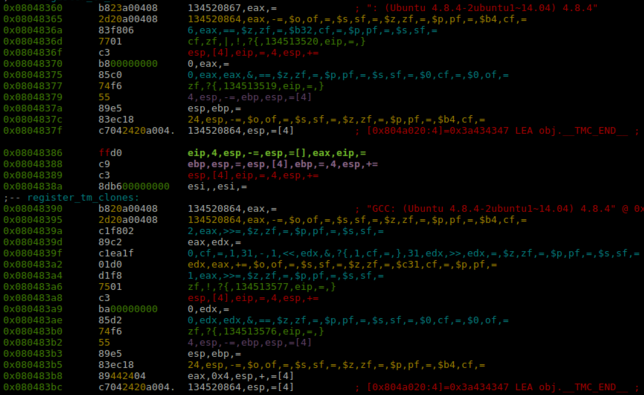
\includegraphics[width=0.49\textwidth]{src/img/disassembleEsil.png}\label{fig:f2}}
	% \hfill
	\caption{Assembly to ESIL}
	\label{fig:disasEsil}
\end{figure}

\subsection{ESIL VM}
\abbrev{VM}{Virtual Machine}

Radare2 also incorporates a virtual machine for emulating ESIL instructions. The ESIL VM has internal state flags and registers mirroring a real CPU, each emulated instruction having the same effects in the VM as it would on the CPU. This is a crucial component for the gadget classification step as it allows the program to emulate the gadget each instruction at a time and analyze its effects on the machine. Based on the effects each gadget will be assigned into one, or more, categories.

% \todo{maybe insert photo of pd call with esil and emu (better not, too crowded ?)}

\subsection{API Hooks}

An important aspect of emulation is the ability to setup user-defined hooks in the parser, thus allowing custom analysis or behavior to be implemented for the desired instructions without having to modify the parser each time. This works by calling calling the hook function each time an operation is about to be executed.

By default the ESIL VM implements for example hooks like hook_flag_read(), hook_execute(), hook_reg_read(), hook_reg_write() etc., for logging information such as when a register or flag have been read or written, or when a memory address has been accessed. This information is heavily used in the gadget classification as well.

% \todo{maybe insert logging example (too small and irrelevant ?)}

\section{Summarize}
\label{sec:sumup}

To sum up, I decided to use the Radare2 Framework for my project because it provides the following tools and features:
\begin{itemize}
	\item It contains a mature ROP gadget searching tool
	\item Provides an Intermediate Language and Virtual Machine for emulation and analysis
	\item Fully cross platform thanks to ESIL VM
	\item Open source code
	\item Continuously improving, with new Git commits each day
	\item Active and friendly community
\end{itemize}



